\resourceheading{5}{Every-Day Personalized Science Souvenir}{Student learning portrait, recognition, memory \& communication continuity\par}{Students, families, teachers \& camp partners}{Implemented EDU486 personalized souvenirs, student memos, and reviewed activity evidence}

\vspace{-0.5cm}
\toolsection{The Existing Camp Artifact}

The video memo preserves an immediate learner account, and the personalized souvenir carries that account into memory and family conversation. The Invisible Invaders team paired a child-forward activity image with the learner's contribution, field-memo thinking, science moves, traceable evidence, why the learning mattered, and what remained unconfirmed. The visual message was direct: \textit{``This is you doing science.''} The product recognized authorship without turning a photograph into proof of understanding \citep{campEvidence2026}. A learner could revisit the day's experiences, point to a mission, retell what they did or learned, and use the visual record when words alone were difficult. The reviewed archive preserves completed souvenirs for every day, including one Day 5 image for each assigned youth.

\toolsection{The Completed Souvenir}

\begin{center}

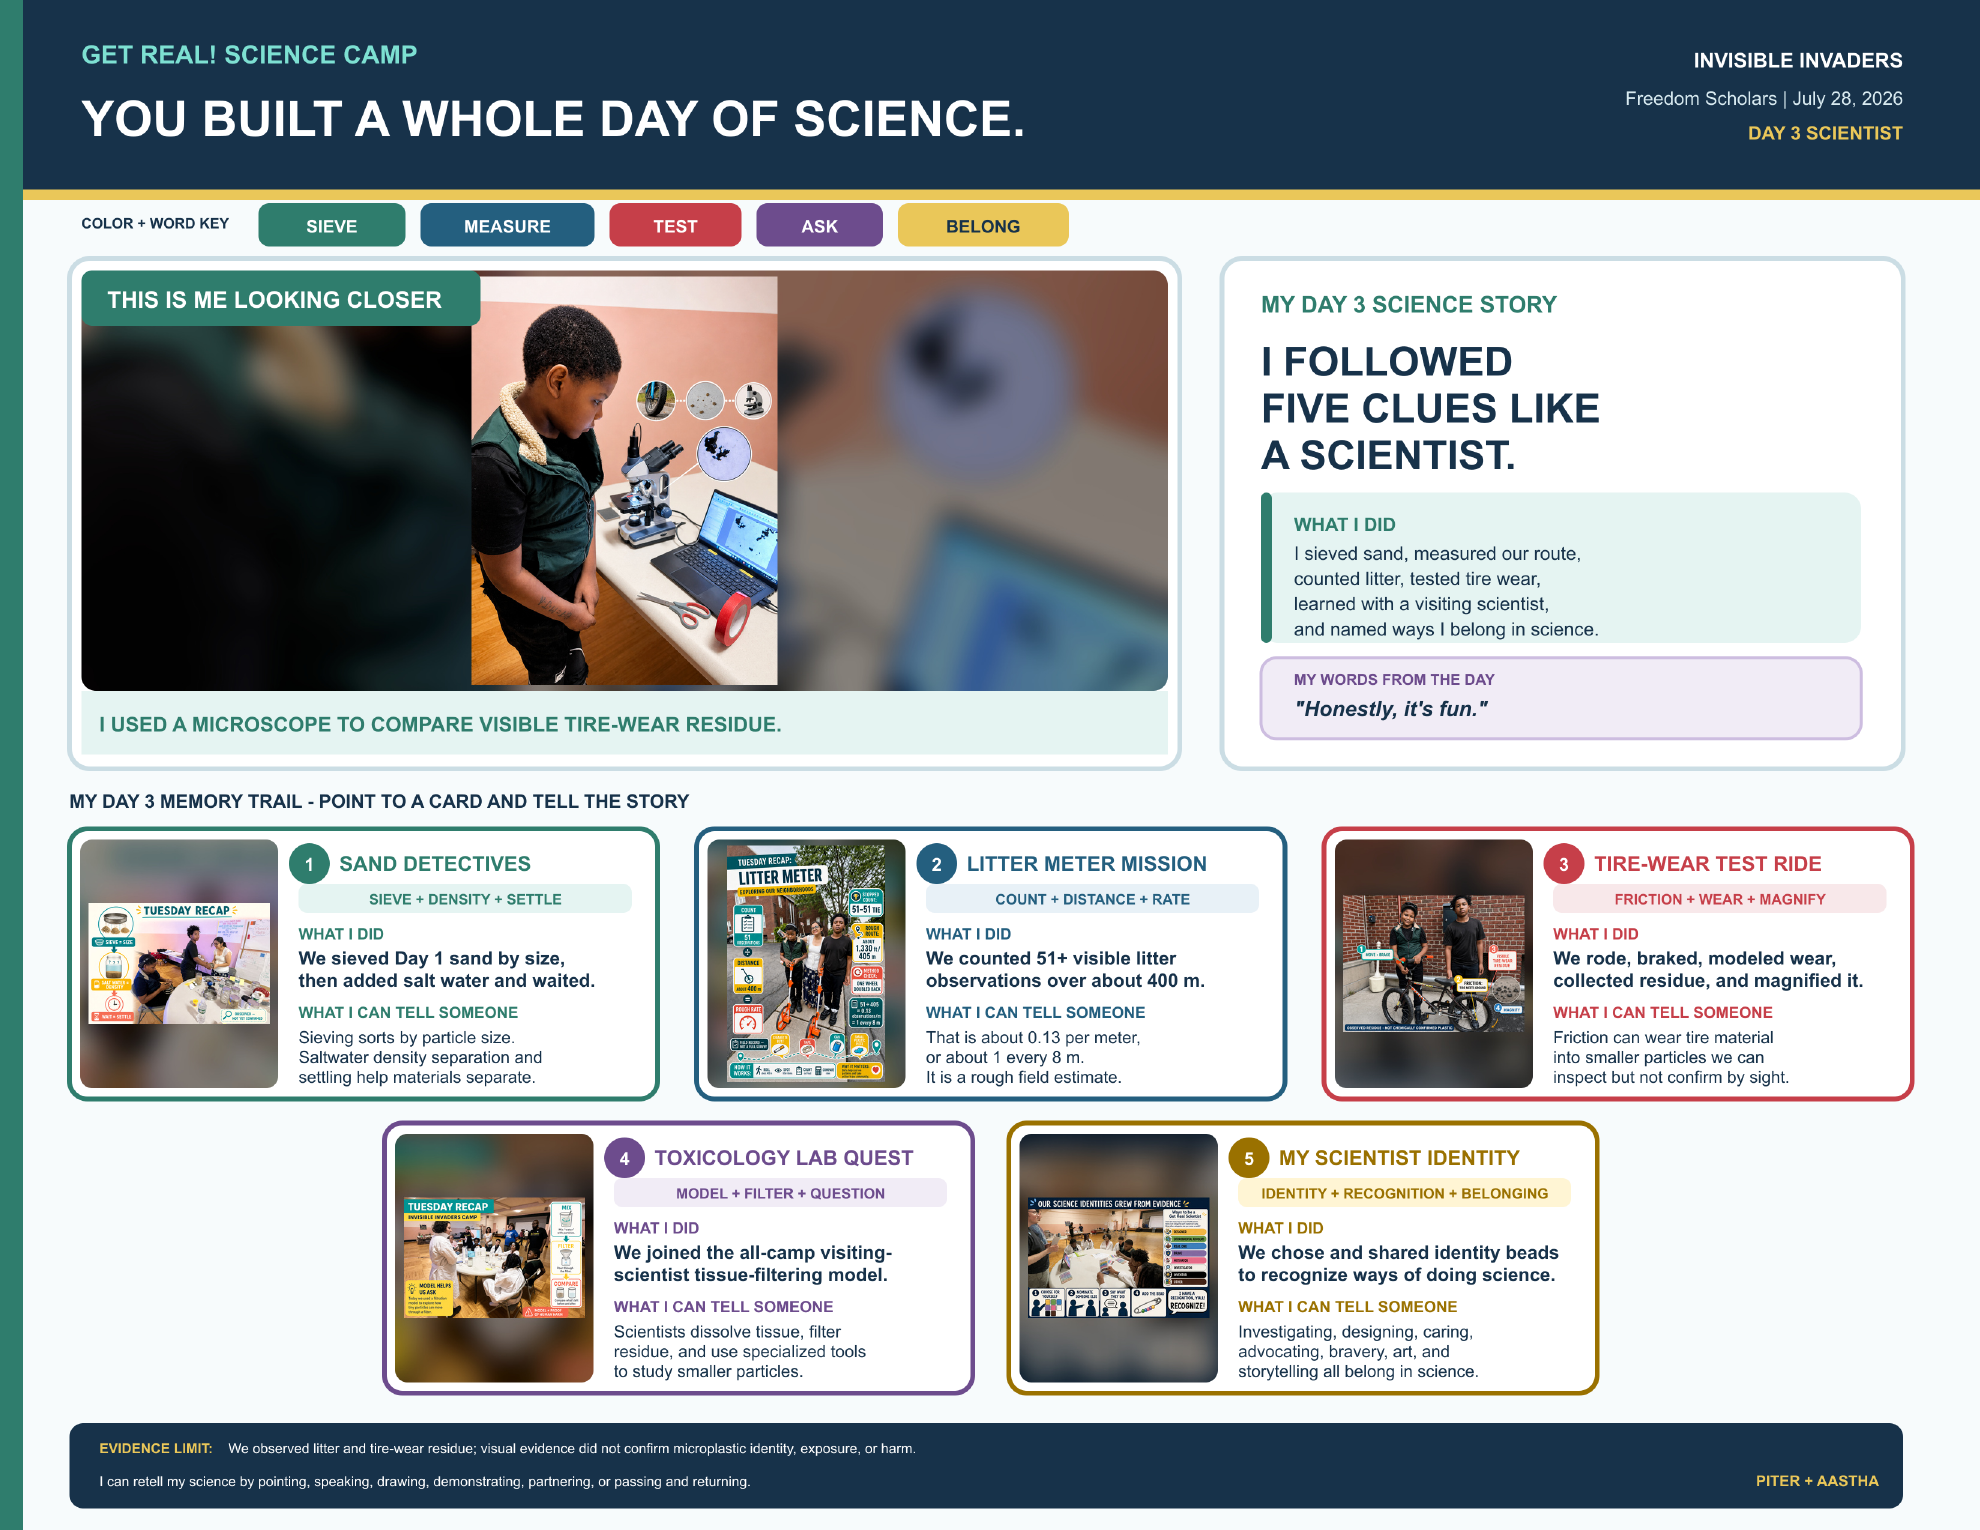
\includegraphics[
  width=0.92\textwidth,
  keepaspectratio
]{assets/artifact-previews/souvenir-day3-example.png}

\parbox{0.92\textwidth}{\centering\small
\textbf{\color{DeepNavy}Public-safe Day 3 souvenir.}
The completed artifact brings together the learner in action, a transcript-grounded science story, five activity memories, the learner's own words, multiple communication routes, and an explicit evidence limit. It functions as both recognition and a reusable memory aid for retelling the learning to teachers, families, or partners.}

\end{center}

\newpage
\toolsection{Build One After Each Activity Day}

\begin{enumerate}
	\item \textbf{Assemble the evidence set:} activity record, student memo or artifact, reviewed photographs, team notes, and the learning goal.
	\item \textbf{Start with the learner's contribution:} identify what the young person chose, noticed, made, changed, asked, explained, or helped the group do.
	\item \textbf{Separate evidence levels:} mark exact words, artifact language, documented action, team-level evidence, adult interpretation, and uncertainty.
	\item \textbf{Select and compose together:} choose the image and idea; add the science story, moves, evidence, significance, and limit; offer caption, translation, retake, and no-photo routes.
	\item \textbf{Review, share, and reuse:} check identity, attribution, quotation, permission, and audience; next day, invite the learner to point, tell, correct, extend, or decline the story.
\end{enumerate}

\toolsection{Evidence-to-Action Review}

% \small
\renewcommand{\arraystretch}{1.00}
\setlength{\tabcolsep}{4pt}
\begin{tabularx}{\textwidth}{>{\bfseries\RaggedRight\arraybackslash}p{1.20in} >{\RaggedRight\arraybackslash}p{2.65in} >{\RaggedRight\arraybackslash}X}
\rowcolor{MidTeal}
\color{white}Souvenir Signal & \color{white}Interpret Carefully & \color{white}Adult Follow-Through \\
Student words & Preserve the learner's meaning; do not polish uncertainty away & Reuse the question, preference, or connection in the next lesson \\
\rowcolor{SoftGray}
Documented action & Participation may be visible without proving the learner's full understanding & Ask the learner what the action meant and offer another way to demonstrate thinking \\
Preference or boundary & Liking, refusing, passing, or requesting change is communication & Change material, role, pace, sensory route, or audience when feasible \\
\rowcolor{SoftGray}
Team contribution & Credit individual influence without claiming the whole team's product & Name both the student's move and the shared work \\
Evidence gap & ``Still to test'' is part of scientific competence, not failure & Carry the uncertainty into the recap and next investigation \\
\end{tabularx}
\normalsize

\toolsection{Puzzle Plan and EQUITAS in Practice}

The Puzzle Plan joins the student's account, observable action, work product, team record, and scientific context without allowing one piece to define the learner. EQUITAS asks who selected the image and story, whose language was edited, whose quieter contribution disappeared, and whether the artifact changes adult memory while celebrating the child. Used this way, the souvenir supports communication and behavior by making competence, boundaries, curiosity, and participation routes visible before a deficit story replaces them.

\reflectionbox{\textbf{Artifact proof:} the private handoff contains reviewed personalized souvenir PDFs, activity images, and source-video indexes. Day 5 is explicitly limited to photographs and a same-session clean transcript; it has no source video. The souvenir system preserves that distinction and never upgrades an attractive visual into stronger evidence \citep{campEvidence2026}.}

\adaptationbox{A souvenir can become a reward, comparison chart, or privacy violation if adults control every choice. Never reserve it for compliance or fluent speech. Offer photo-free, name-free, home-language, AAC, audio, tactile, or student-created versions. Use identifiable copies only within the program's signed consent and approved educational audience.}

\sourcebox{Personalized souvenir archive \citep{campEvidence2026}; communicative competence \citep{jorgensen2018competence}; first-hand perspectives \citep{gardner2017firsthand}.}